\documentclass[peerreview]{IEEEtran}
\usepackage{cite} % Tidies up citation numbers.
\usepackage{url} % Provides better formatting of URLs.
\usepackage[utf8]{inputenc} % Allows Turkish characters.
\usepackage{booktabs} % Allows the use of \toprule, \midrule and \bottomrule in tables for horizontal lines
\usepackage{graphicx}
\usepackage{xcolor}

\usepackage{listings}

\definecolor{mygreen}{rgb}{0,0.6,0}
\definecolor{mygray}{rgb}{0.5,0.5,0.5}
\definecolor{mymauve}{rgb}{0.58,0,0.82}

\definecolor{mylilas}{RGB}{170,55,241}

\lstdefinestyle{CStyle}{
	belowcaptionskip=1\baselineskip,
	breaklines=true,
	frame=L,
	xleftmargin=\parindent,
	language=C,
	showstringspaces=false,
	basicstyle=\footnotesize\ttfamily,
	keywordstyle=\bfseries\color{green!40!black},
	commentstyle=\itshape\color{purple!40!black},
	identifierstyle=\color{blue},
	stringstyle=\color{orange},
}

\lstdefinestyle{Matlab}{
    language=Matlab,
	belowcaptionskip=1\baselineskip,
    frame=L,
    xleftmargin=\parindent,
    basicstyle=\footnotesize\ttfamily,
    breaklines=true,
    morekeywords={matlab2tikz},
    keywordstyle=\color{blue},
    morekeywords=[2]{1}, keywordstyle=[2]{\color{black}},
    identifierstyle=\color{black},
    stringstyle=\color{mylilas},
    commentstyle=\color{mygreen},
    showstringspaces=false,
    numberstyle={\tiny \color{black}},
    numbersep=9pt,
    emph=[1]{for,end,break},emphstyle=[1]\color{red},
}

\hyphenation{op-tical net-works semi-conduc-tor} % Corrects some bad hyphenation 

\begin{document}
%\begin{titlepage}
% paper title
% can use linebreaks \\ within to get better formatting as desired
\title{System on Chip Architecture \\ Lab 2 Report}

% author names and affiliations

\author{Daniele Castro S253244\\
System-on-chip architecture\\
Politecnico of Turin\\
}
\date{26/12/2018}

% make the title area
\maketitle
\tableofcontents
\listoffigures
%\end{titlepage}

\IEEEpeerreviewmaketitle
\begin{abstract}
In this lab I implemented a simple function generator using the MCU STM32F051R8 on the discovery board. Doing that I tried as much as I could to use MCU hardware support so that the final work performs the best. Surely the output signal has some analog hardware limitations: it can only output signals in the range of 0v and 3.3v. To shift and amplify it, for instance, between -1v and +1v an analog output circuitry is required and I made it.
\end{abstract}
\section{Introduction}
Here is a small figure that better explains what this function generator does using hardware support:
\begin{figure}[!ht]
\centering
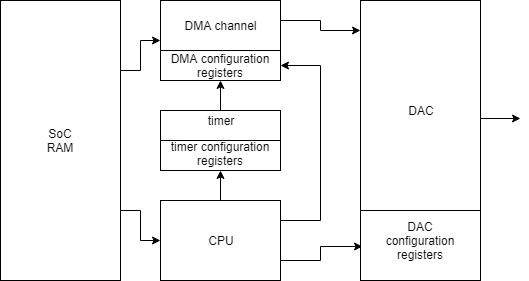
\includegraphics[width=0.8\columnwidth]{DAC} 
\caption{block diagram}
\label{fig_sim}
\end{figure}
\\It's easy to understand that CPU only configures these peripherals. That means that, after the initialization stage, can be switched off to drain less current. Infact it is what i did putting the CPU in STOP mode.
\section{Background}
The STM32F051R8 has 12-bit DAC (Digital to Analg Converter). That means that it can quantize an analog signal with $2^{12}-1$ digital unsigned values. DMA channel 13 moves signal frames stored in memory to the DAC without CPU usage and timer TIM2 triggers the DAC to output a frame at $1/(1/(48*(10^{6}))*((2^{8})-1)) = 188.2352941$MHz. Since prescaler and postscaler are disabled, TIM2 increments his count register at system frequency that is 48MHz.
\section{Proposed Solution}
Depending on the application, of course, this laboratory can be made in different ways. For instance there is the possibility to do not use both timer and DMA and to do everything with CPU. This implementation can have some advantages like power saving since we are using less peripherals and can be also implemented in cheaper hardware that hasn't got any DMA channel like some 8-bit micro controllers. But it has the disadvantage that is limited in the maximum frequency at which samples can be output and code occupies much more memory. So, normally a good approach is to choose hardware to use dependently on what we have to do and, when present, use all the possible peripherals instead of emulating them in software.
Stop mode is the best to put the CPU in after the initialization process since it does not disable peripherals and powers off only the CPU core.
In terms of code written I only made an header file called "waveform" that contains samples numerical values I calculated  using a MATLAB script:
\begin{lstlisting}[style=Matlab]
clear
clc
unit = ((2*pi)/1024);
y = 0:unit:(2*pi)-unit;
t = sin(y);
t = ((t+max(t))/(2*max(t)))*hex2dec('FFF');
numel(t)
t = int16(t);
plot(t);
M = vec2mat(t, 16)
numel(M)
F = string(M);
F(:, :, 1) = F(:, :, 1)+','+' ';
H = char(F);
dlmwrite('values_1024.txt', H,'delimiter','');
\end{lstlisting}
this specific script outputs in a file sample unsigned values for a full sine wave period so that, since DMA is configured in circular mode, at the and of the sample windows DMA pointer will start again from the beginning of the window. Changing \lstinline[style=Matlab]{sin(y)} with \lstinline[style=Matlab]{square(y)} this script will generate samples for a square wave. Both of these waves samples are saved in the file  "waveform". Here I show their definitions:
\begin{lstlisting}[style=CStyle]
#include <stdint.h>

//#define SQUARE //comment for sinewave

#ifdef SQUARE
extern const uint16_t Square12bit[1024];
#else
extern const uint16_t Sine12bit[1024];
#endif
\end{lstlisting}
\lstinline[style=CStyle]{#ifdef} statements are put only to make the possibility to choose, only on compile time, wether to output a square wave or a sine wave. At run time only Escalator wave form can be changed with the current one previously selected by pressing the user button, but since the button pressure is CPU handled when we go in stop mode this event can't be handled anymore and, so, waveform can't be changed at run time. Here is the code I wrote:
\begin{lstlisting}[style=CStyle]
...
else
{
	printf("Entered in StopMode\n\r");
	StopMode_Measure();
	USART2_init();
	printf("Exited from StopMode\n\r");
}
...
\end{lstlisting}
other small modifications I made are in the DMA buffer lenght. I put some defines and I recalculated period samples with the MATLAB script above:
\begin{lstlisting}[style=CStyle]
...
		#ifdef SQUARE
DMA_InitStructure.DMA_MemoryBaseAddr = (uint32_t)&Square12bit;
		#else
DMA_InitStructure.DMA_MemoryBaseAddr = (uint32_t)&Sine12bit;
		#endif
...
DMA_InitStructure.DMA_BufferSize = 1024;
...
\end{lstlisting}
As usual I also configured the serial port to output debug messages so that what waveform is going to be output can be known even before plugging the oscilloscope:
\begin{figure}[!ht]
\centering
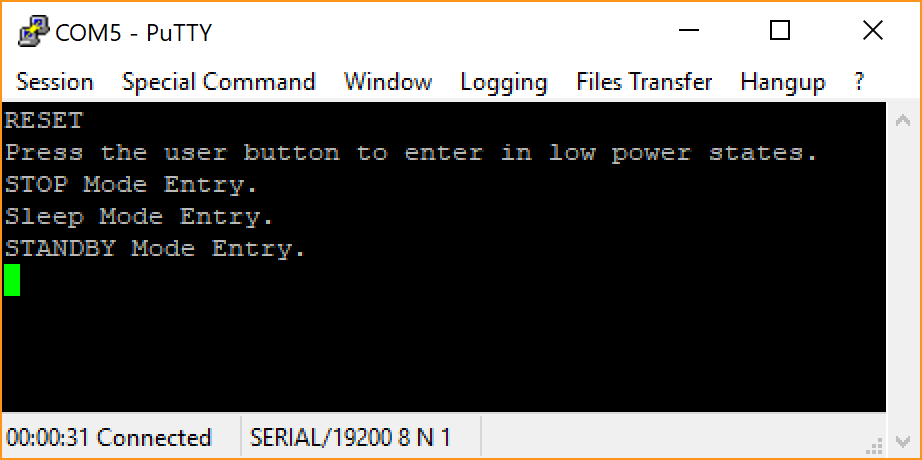
\includegraphics[width=0.8\columnwidth]{serial} 
\caption{serial console}
\label{fig_ser}
\end{figure}
\section{Results and discussion}
The oscilloscope waveform output of the three waveforms are here displayed. Of course there are noise distortions but signal is well accurated since we have a lot of samples representing a single period:
\begin{figure}[!ht]
\centering
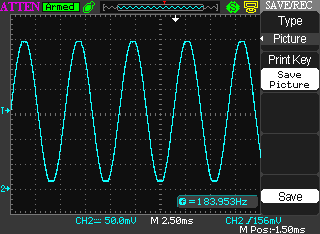
\includegraphics[width=0.8\columnwidth]{sine} 
\caption{sine waveform}
\label{fig_sine}
\end{figure}
\begin{figure}[!ht]
\centering
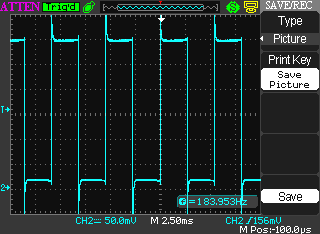
\includegraphics[width=0.8\columnwidth]{square} 
\caption{square waveform}
\label{fig_square}
\end{figure}
\begin{figure}[!ht]
\centering
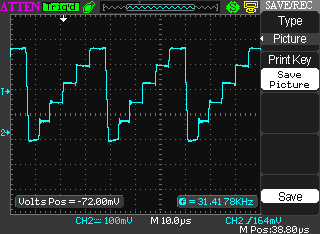
\includegraphics[width=0.8\columnwidth]{escalator} 
\caption{escalator waveform}
\label{fig_escalator}
\end{figure}
\\I also made tests with my hand made analog voltage shifter I was speaking in the abstract:
\begin{figure}[!ht]
\centering
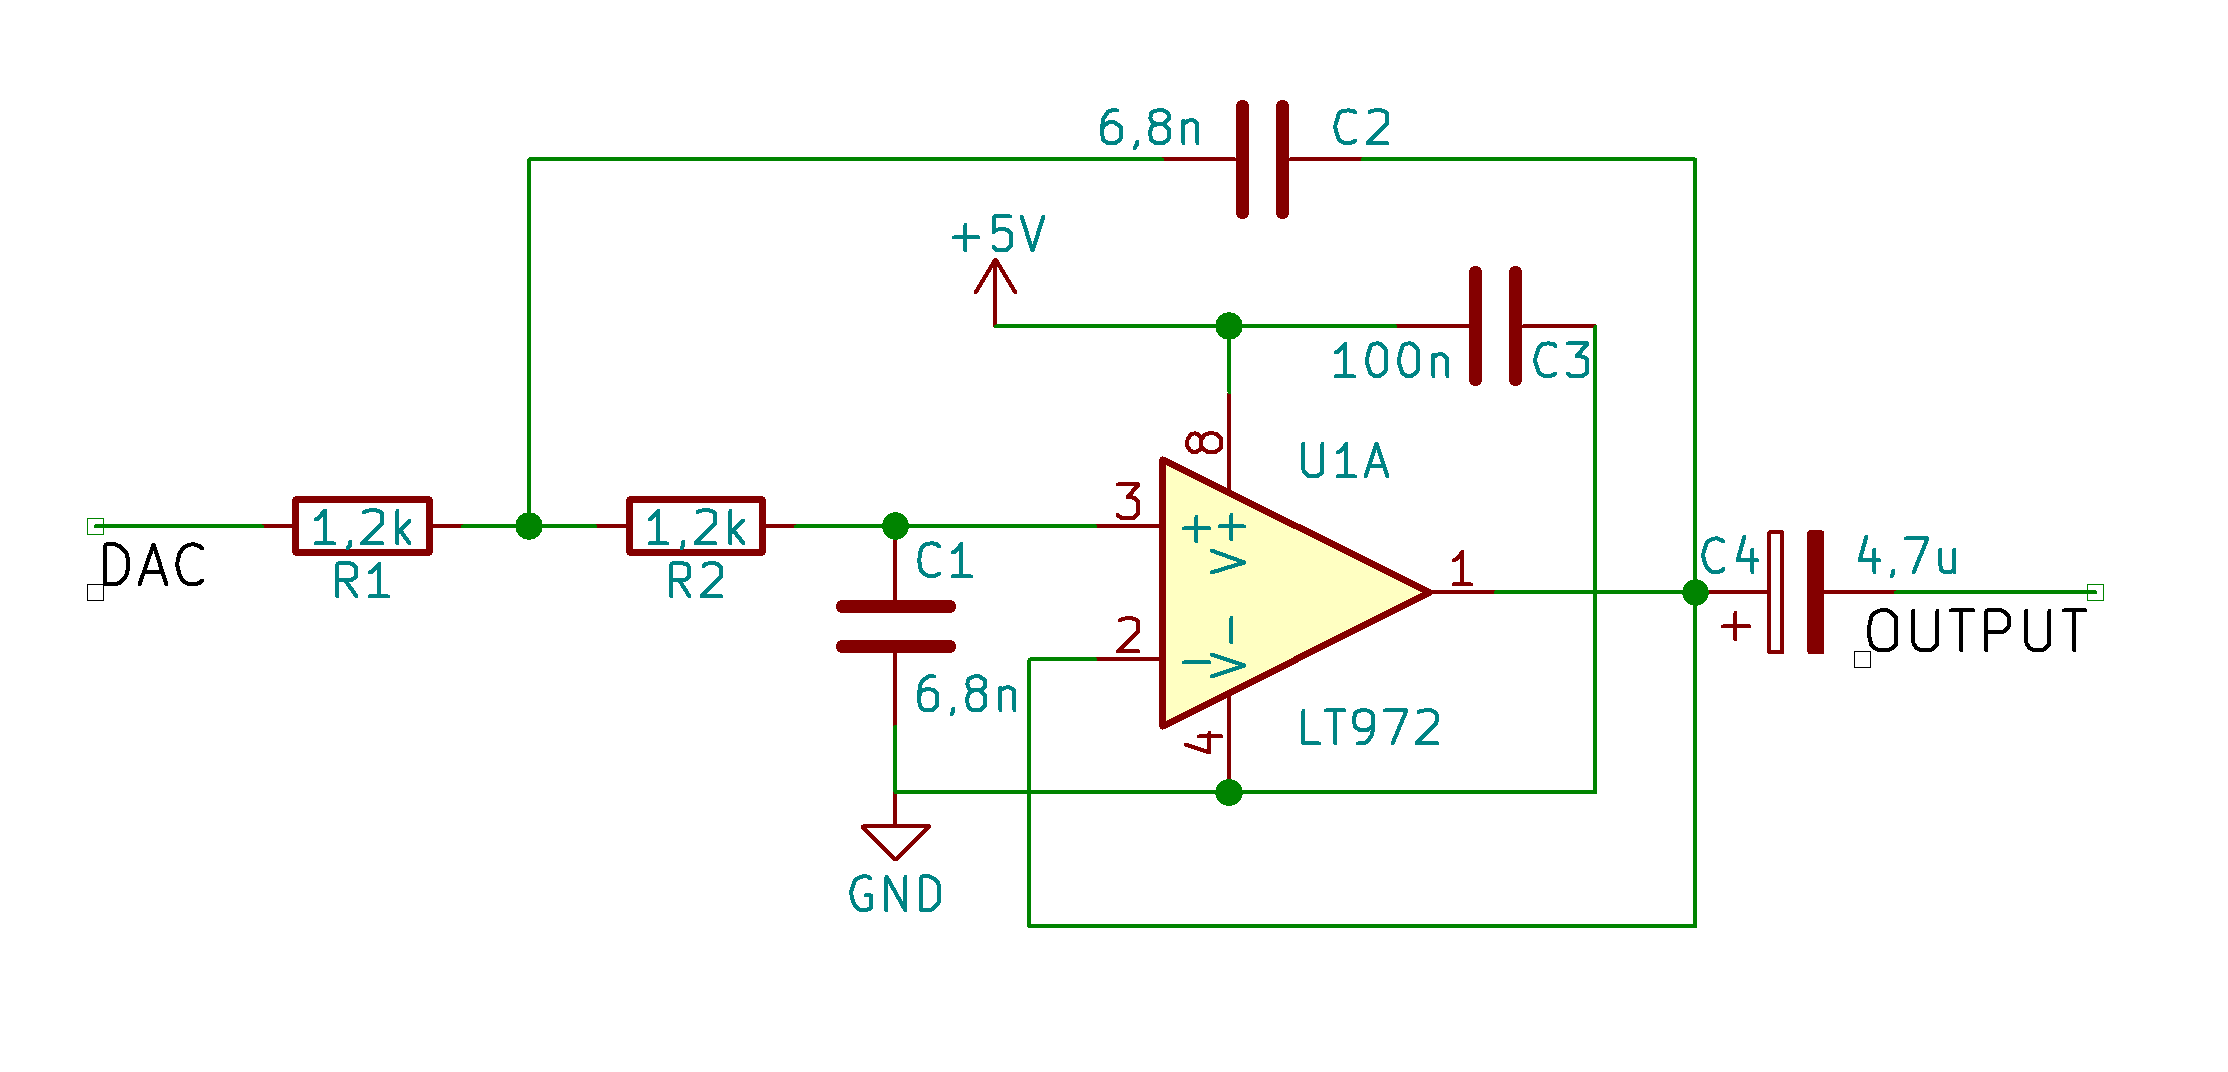
\includegraphics[width=0.8\columnwidth]{diagram} 
\caption{analog circuit diagram}
\label{fig_diagram}
\end{figure}
\section{Results and discussion}
\label{tab:template}
in this way I can connect directly to my PCs audio acquisition peripheral everything and print signals in the range of 20MHz - 20KHz. I saw that waves I modified are at 183Hz
\section{Conclusions}
In this discussion I matched the assignment requests and, as an extra, I also made an analog voltage shifting circuitry.
\end{document}